% !TeX root = main.tex

% Requires in the preamble:
% \usepackage{amsmath}
% \usepackage{graphicx}
% \usepackage{multirow}
%
% Suggested placement:
% Insert after the reduced-order body--tail model section, or merge with the
% existing gravity-loaded U-bending section. Figure files should be copied to
% the paper's figures/ directory, or the paths below should be edited.

\section{IMAGE-BASED BODY--TAIL RECONSTRUCTION RESULTS}
\label{sec:body_tail_reconstruction_results}

The reduced-order model was evaluated on five representative frames extracted from the body--tail actuator experiments. Two top-view frames were used for the crossed-channel S-shaped mode, corresponding to opposite assignments of the pressurized chamber pair. Three side-view frames were used for the uncrossed-channel vertical U-shaped mode, corresponding to the assembled robot with no added tip load, with a 2.0 g tail-tip metal nut, and with a 5.7 g tail-tip metal nut. In all cases, the pressure display was included in the image frame, and the body and tail centerlines were digitized manually. Each segment was fitted by a circular arc, from which the signed bending angles, curvatures, bending transmission ratio, and reconstruction error were computed.

\subsection{Horizontal S-Shaped Reconstruction}

Figure~\ref{fig:s_shape_reconstruction_results} shows the reconstructed crossed-channel S-shaped postures. The first actuation direction produced a body bending angle of $-104.9^\circ$ and a tail bending angle of $91.2^\circ$ at 11.1 kPa, giving a bending transmission ratio of $\eta=0.869$. The second actuation direction produced a body bending angle of $90.8^\circ$ and a tail bending angle of $-92.9^\circ$ at 10.2 kPa, giving $\eta=1.023$. In both cases the product of the signed curvatures was negative, confirming the opposite-curvature condition for the S-shaped mode,
\begin{equation}
  \kappa_b\kappa_t < 0 .
  \label{eqn:s_shape_result_condition}
\end{equation}
The fitted arcs closely followed the picked centerline points, with root-mean-square errors below 0.24 mm for all body and tail segments in the S-shaped reconstructions. These results show that the crossed pneumatic routing produces the intended lateral S-shaped body--tail deformation in both actuation directions.

\begin{figure}[tb]
  \centering
  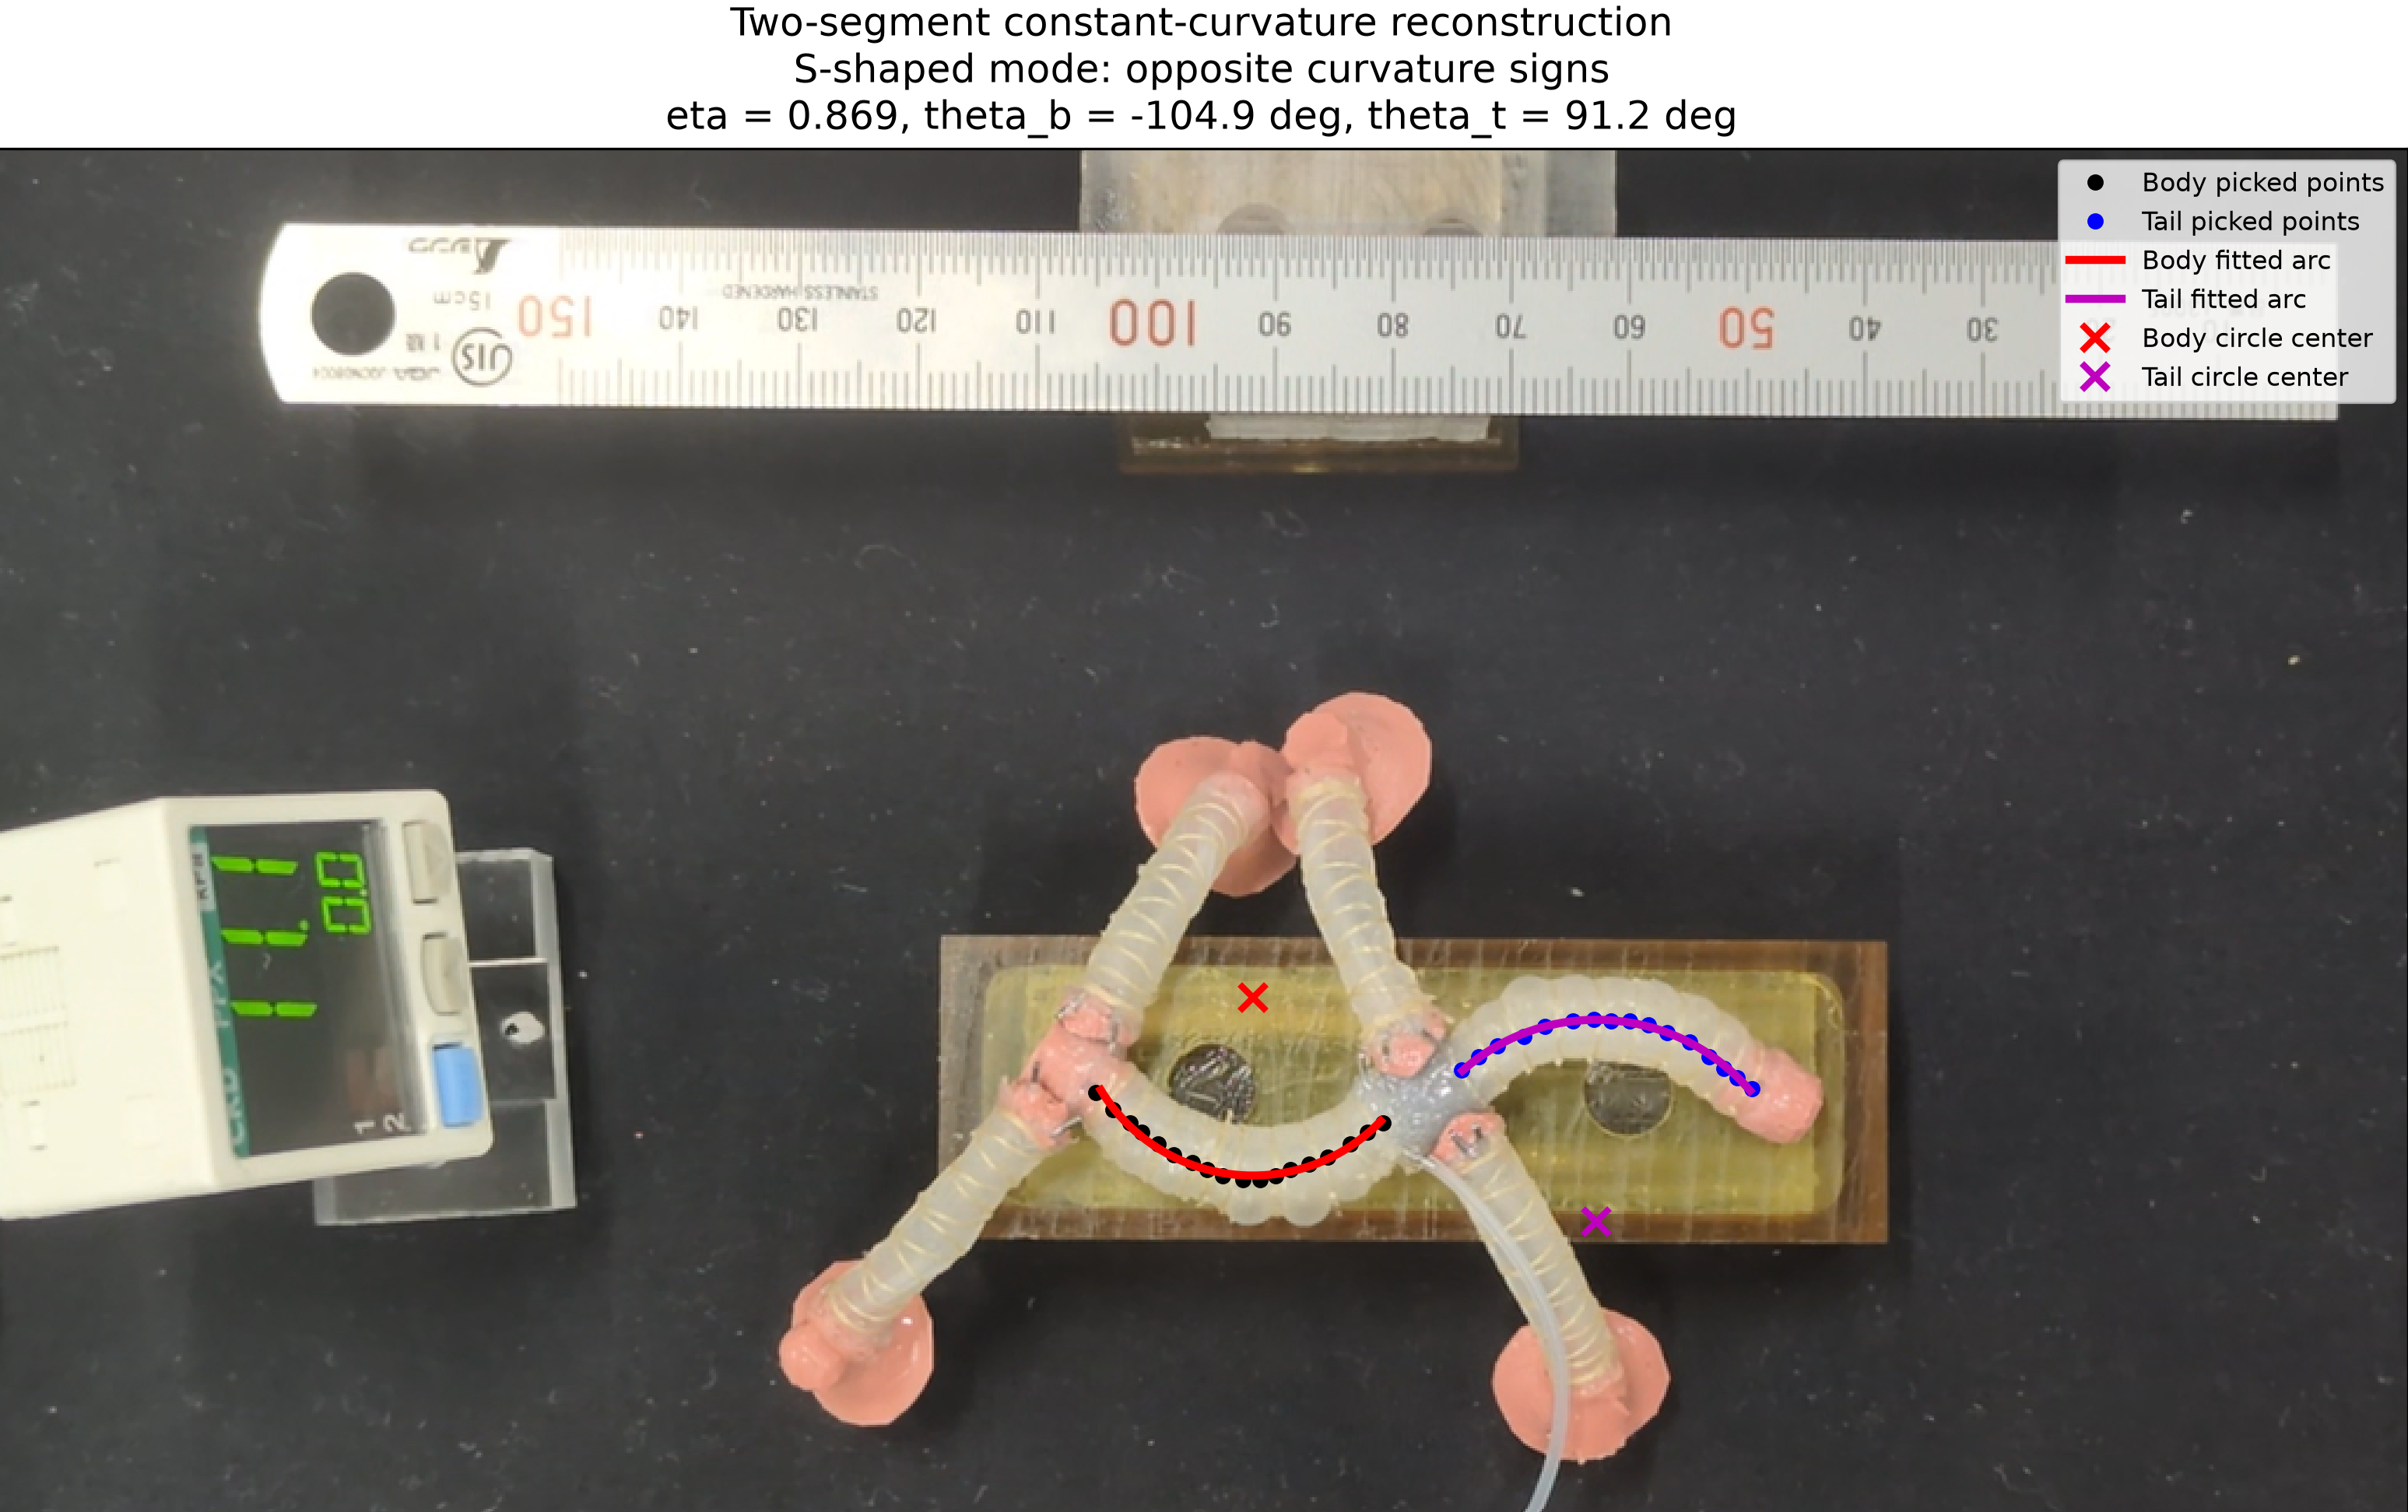
\includegraphics[width=0.49\linewidth]{figures/Sbodydown11.1_reconstruction_overlay.png}
  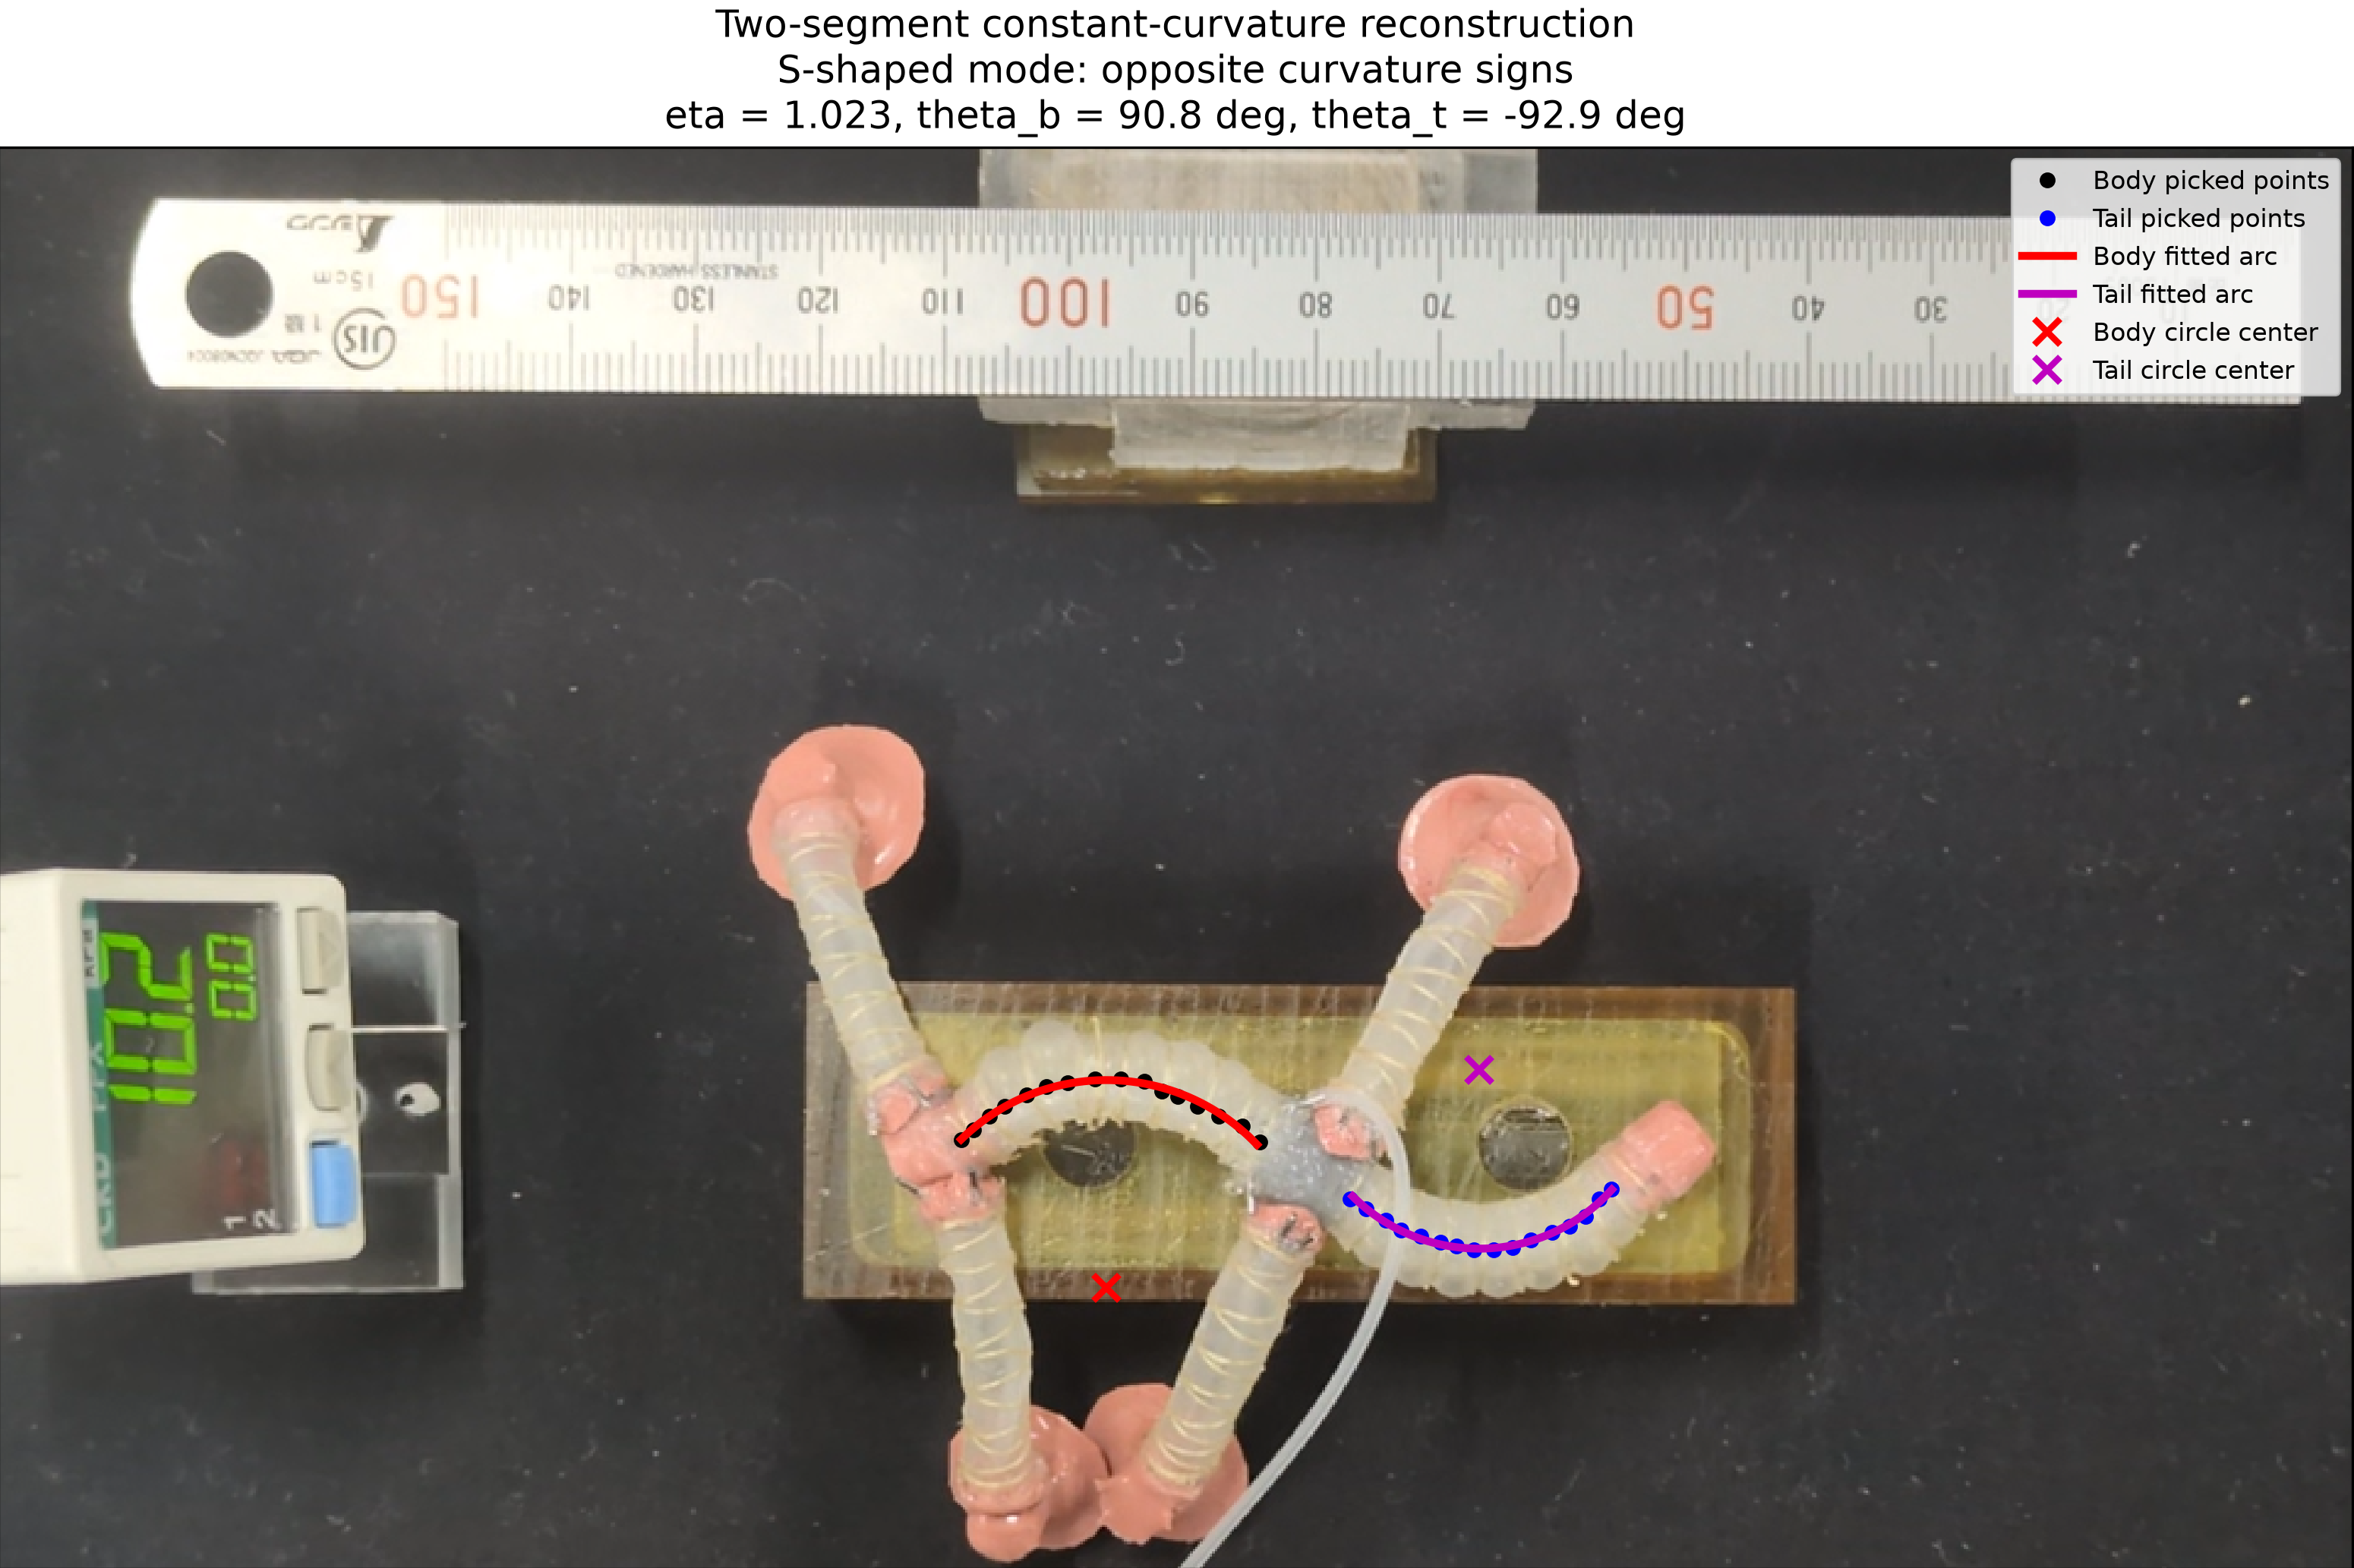
\includegraphics[width=0.49\linewidth]{figures/Sbodyup10.2_reconstruction_overlay.png}
  \caption{Image-based reconstruction of the horizontal S-shaped body--tail mode. (a) Crossed-channel actuation at 11.1 kPa produced $\theta_b=-104.9^\circ$, $\theta_t=91.2^\circ$, and $\eta=0.869$. (b) Opposite actuation at 10.2 kPa produced $\theta_b=90.8^\circ$, $\theta_t=-92.9^\circ$, and $\eta=1.023$. In both cases the signed curvatures have opposite signs.}
  \label{fig:s_shape_reconstruction_results}
\end{figure}

\subsection{Gravity-Loaded U-Shaped Reconstruction}

Figure~\ref{fig:u_shape_reconstruction_results} shows the side-view reconstruction of the vertical U-shaped mode. Since the posterior suction-cup feet were engaged on the substrate, these reconstructions represent gravity-loaded postures of the assembled robot rather than free-space actuator shapes. The posterior-foot support was represented by a projected hinge point, and the front lifting height was measured along the prescribed upward direction.

Without an added tip load, the body bending angle was $66.2^\circ$, while the tail bending angle was $157.4^\circ$ at 10.5 kPa. The resulting bending ratio was $\eta=2.379$, indicating that the distal segment underwent a larger projected curvature than the body in this unloaded U-shaped posture. The measured front height relative to the posterior hinge was $-0.7$ mm, meaning that the selected front point did not rise above the hinge reference in the side-view measurement. This condition therefore provides a baseline gravity-loaded U-shaped deformation, but not a strong front-lifting posture.

With the 2.0 g nut, the body bending angle increased to $93.0^\circ$, the tail bending angle decreased to $66.8^\circ$, and the bending ratio became $\eta=0.718$ at 10.9 kPa. The projected front height increased to 7.2 mm, and the estimated magnitude of the tail-tip gravitational moment about the posterior support was $2.98\times10^{-4}$ N m. However, visual inspection of the video frame showed that the tail also deviated out of the side-view plane. This behavior indicates that the medium tip load did not produce an ideal planar U-shaped response, but instead excited a coupled torsion--bending mode.

With the 5.7 g nut, the body and tail bending angles were $98.5^\circ$ and $63.1^\circ$, respectively, at 11.4 kPa, giving $\eta=0.641$. The projected front height reached 11.1 mm, and the tail-tip gravitational moment increased to $1.51\times10^{-3}$ N m. Although the heavier load increased the moment about the posterior support, the tail motion was more restricted than in the 2.0 g case. This suggests that increasing the rear load can improve the projected front-lifting posture over the tested range, but also changes the loading regime of the tail.

\begin{figure}[tb]
  \centering
  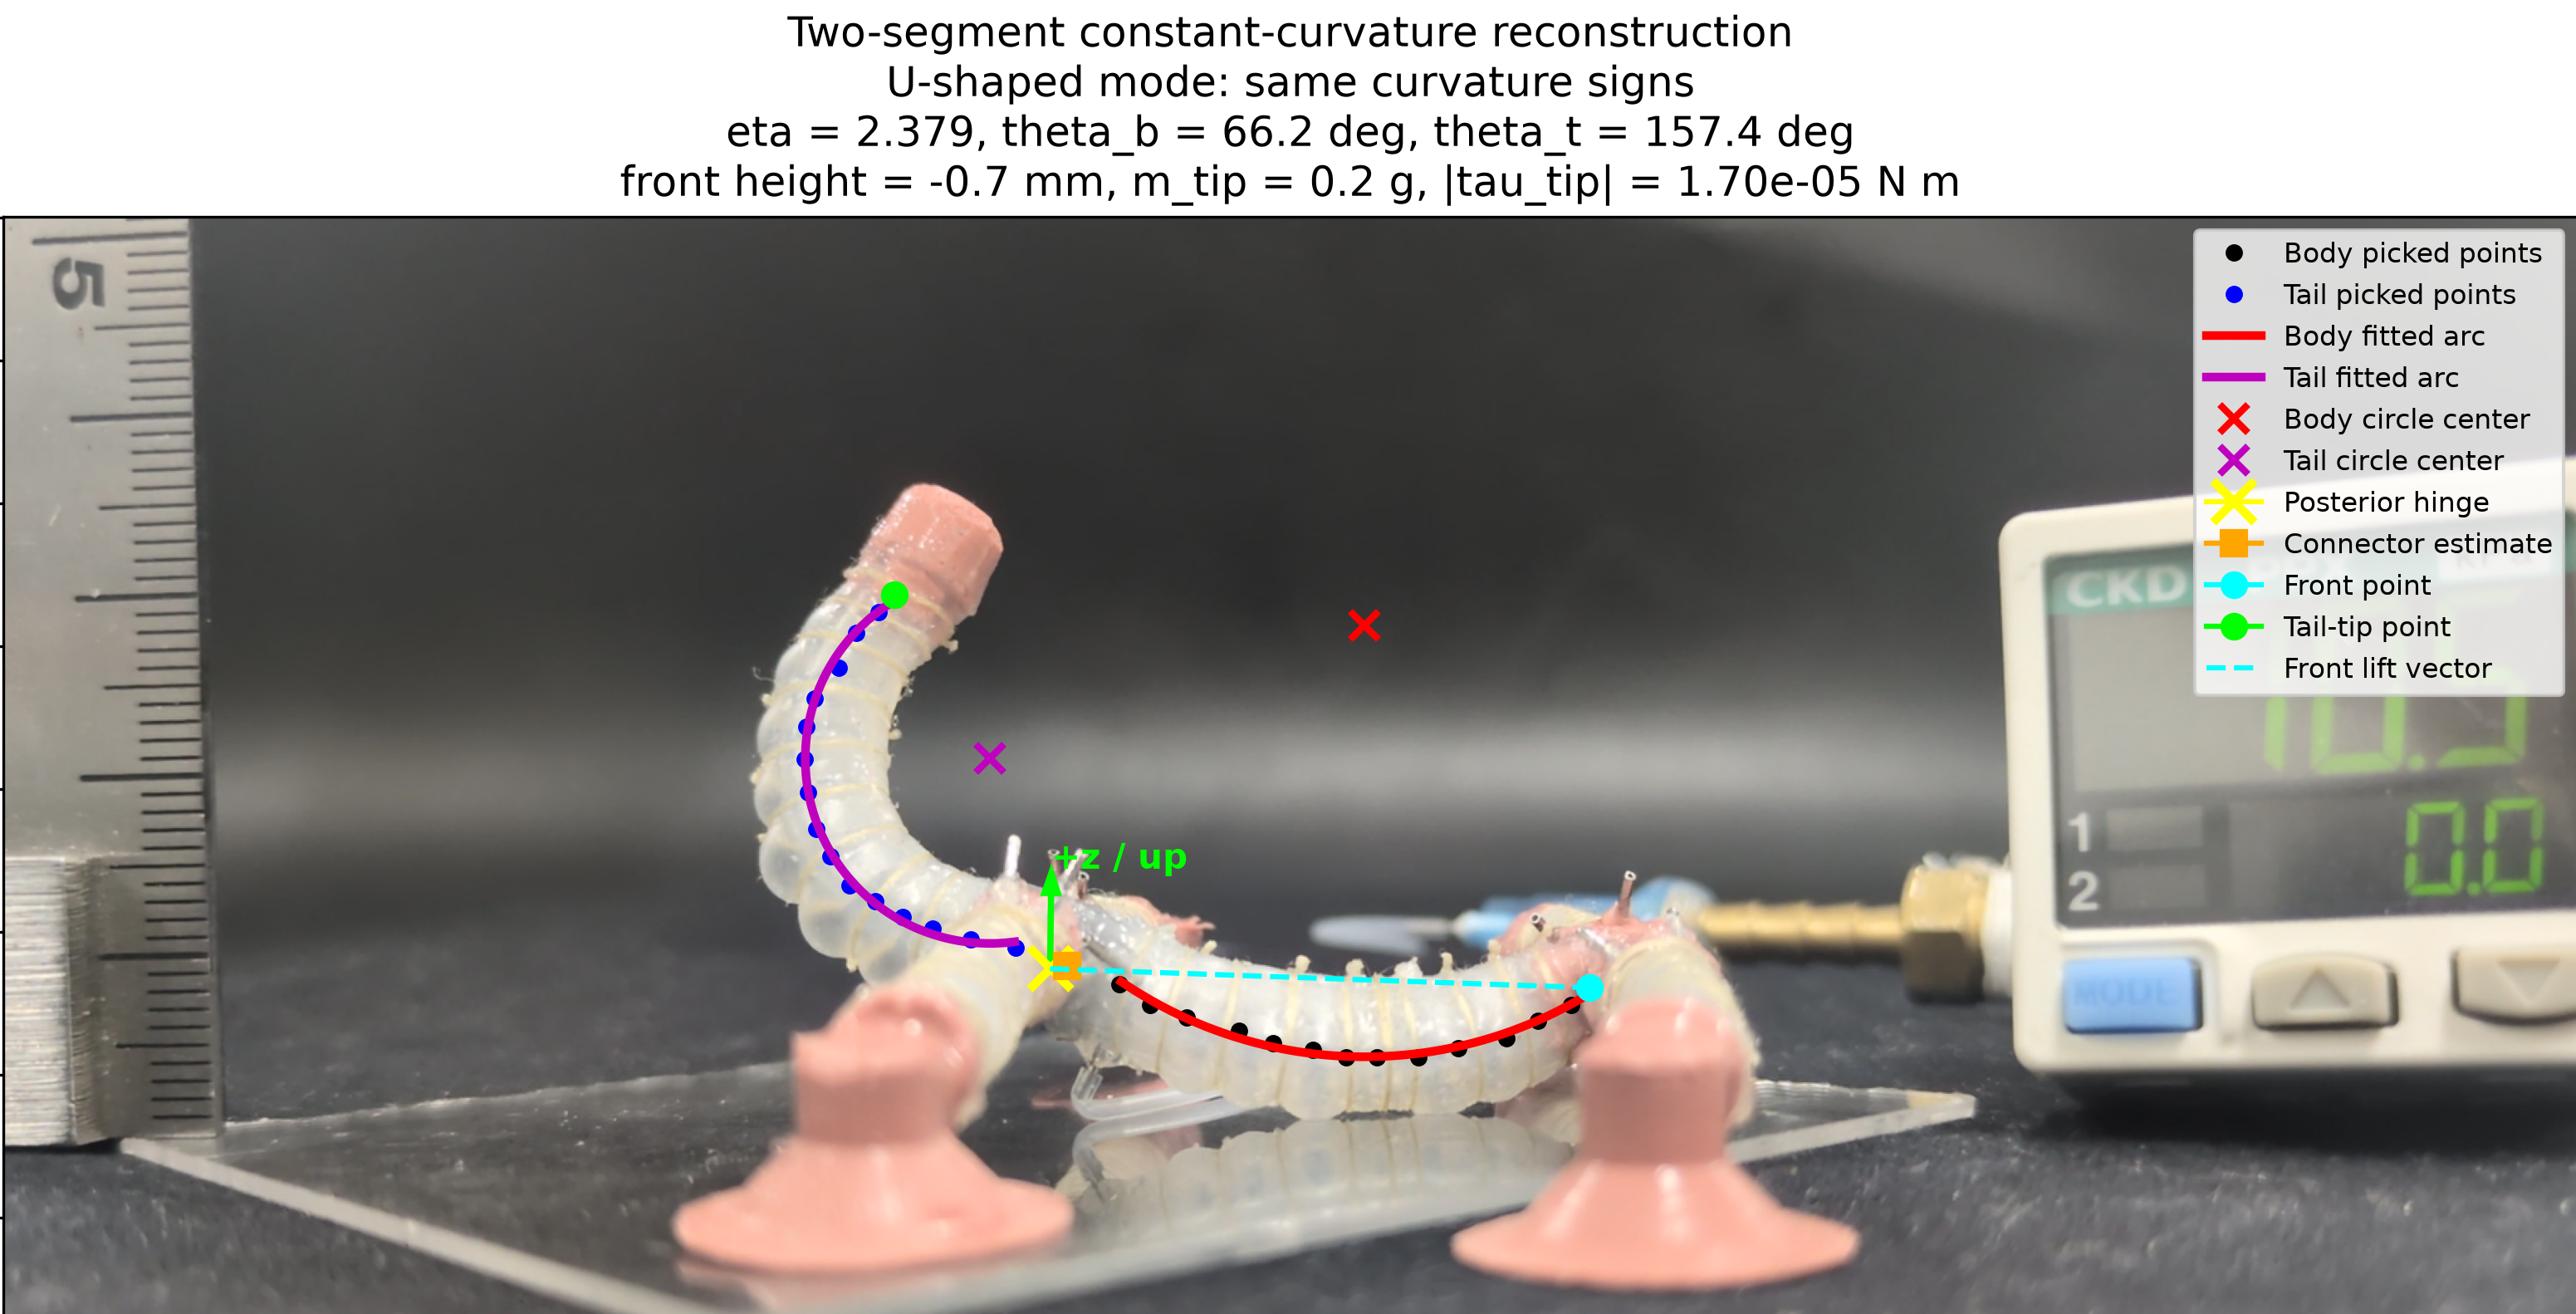
\includegraphics[width=0.32\linewidth]{figures/Unonut10.5_reconstruction_overlay.png}
  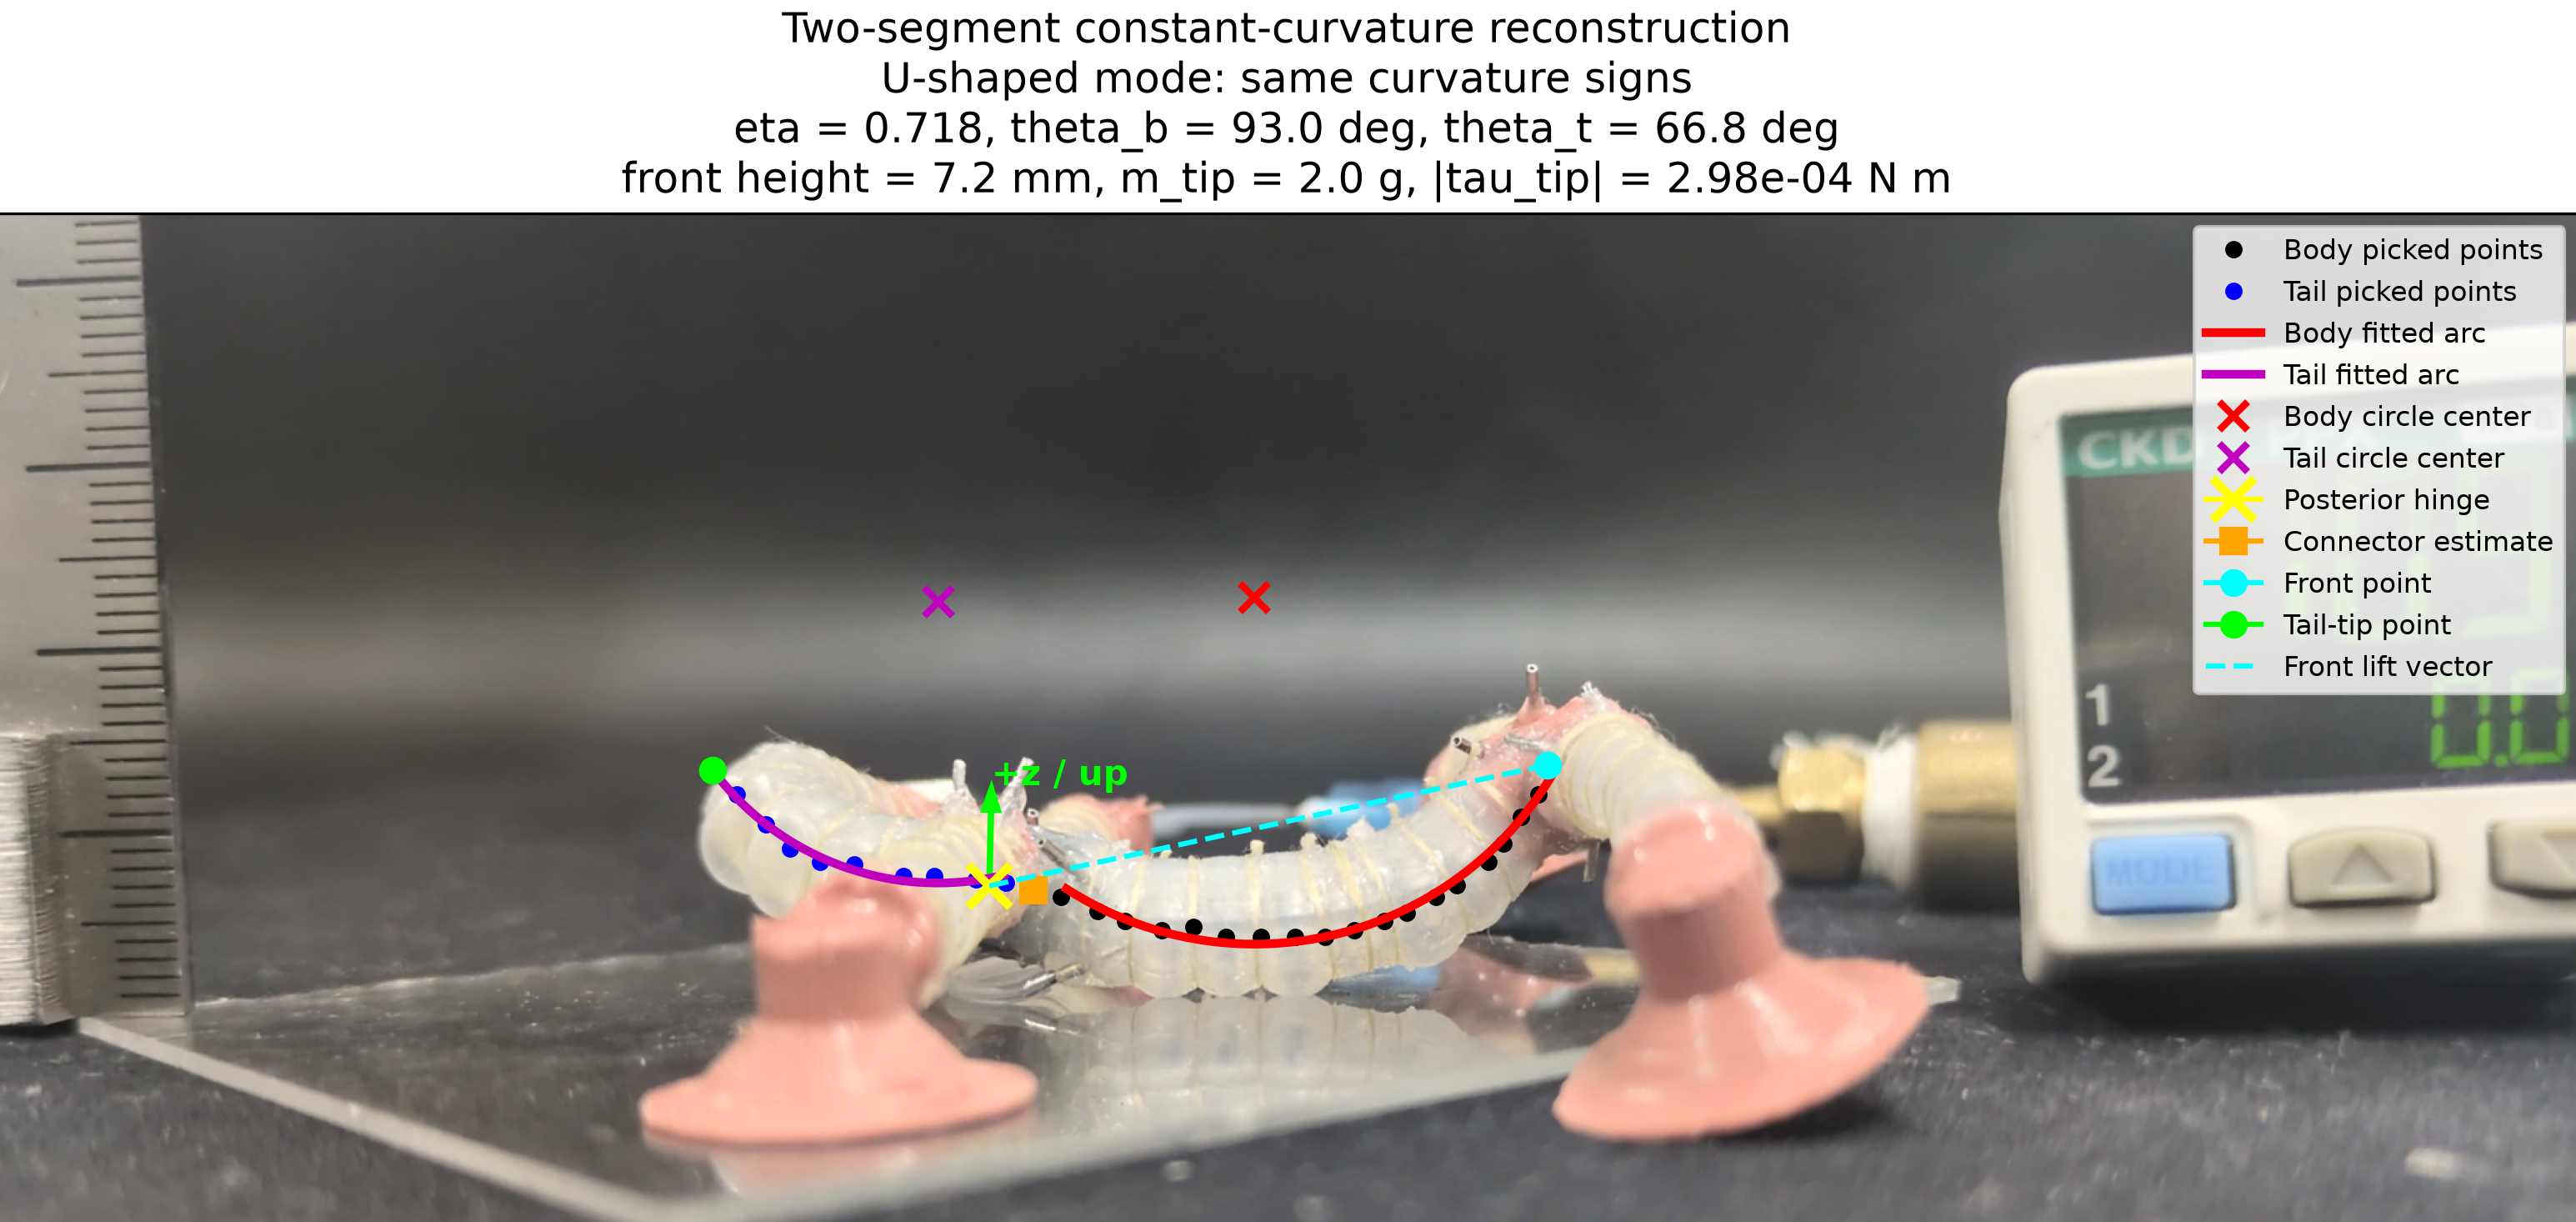
\includegraphics[width=0.32\linewidth]{figures/Usmallnut10.9_reconstruction_overlay.png}
  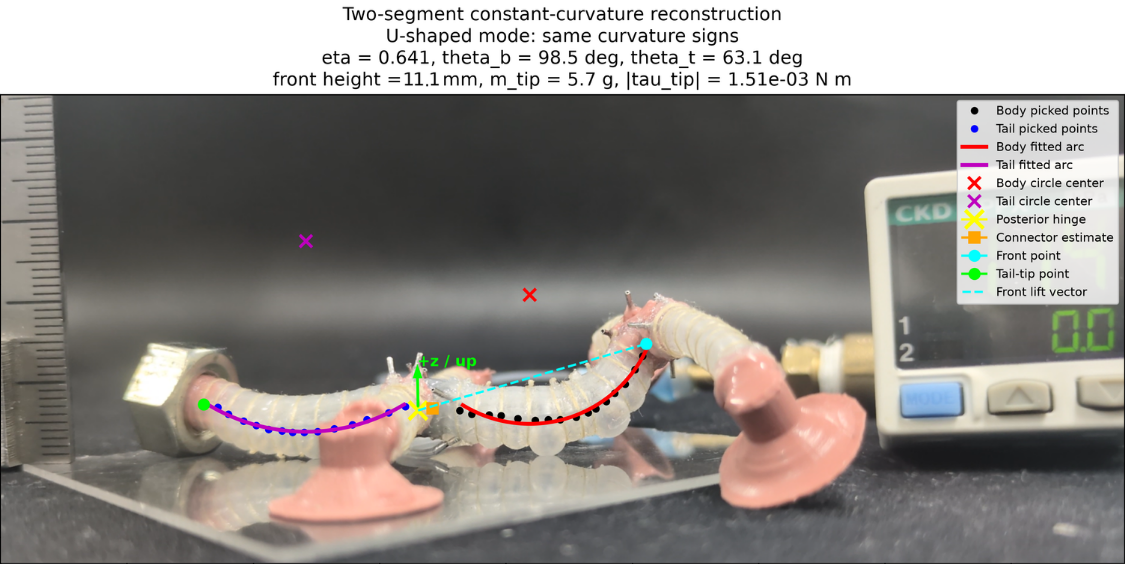
\includegraphics[width=0.32\linewidth]{figures/Ubignut11.4_reconstruction_overlay.png}
  \caption{Image-based reconstruction of the gravity-loaded vertical U-shaped mode. (a) No added tip load at 10.5 kPa. (b) 2.0 g tail-tip nut at 10.9 kPa. (c) 5.7 g tail-tip nut at 11.4 kPa. The posterior suction-cup support, upward direction, front point, tail-tip point, and fitted body--tail arcs are shown in each frame.}
  \label{fig:u_shape_reconstruction_results}
\end{figure}

\begin{table}[tb]
  \caption{Image-Based Reconstruction Results for the Body--Tail Actuator.}
  \label{tab:body_tail_reconstruction_results}
  \centering
  \begin{tabular}{|c|c|c|c|c|c|c|}
    \hline
    Mode & Load & $P$ & $\theta_b$ & $\theta_t$ & $\eta$ & $h_f$ \\
    &  & kPa & deg & deg & -- & mm \\
    \hline
    S & -- & 11.1 & $-104.9$ & $91.2$ & 0.869 & -- \\
    S & -- & 10.2 & $90.8$ & $-92.9$ & 1.023 & -- \\
    U & none & 10.5 & $66.2$ & $157.4$ & 2.379 & $-0.7$ \\
    U & 2.0 g & 10.9 & $93.0$ & $66.8$ & 0.718 & 7.2 \\
    U & 5.7 g & 11.4 & $98.5$ & $63.1$ & 0.641 & 11.1 \\
    \hline
  \end{tabular}
\end{table}

\subsection{Interpretation of the Tip-Load Response}

The U-shaped gravity-loaded results show that the tail-tip load affects not only the magnitude of front lifting, but also the deformation plane of the soft body--tail unit. The planar model assumes that the tail-tip position remains in the side-view plane. If a lateral out-of-plane displacement $y$ develops, the gravitational force of the nut generates an additional torsional moment about the body--tail axis. For a tail-tip position $\mathbf{r}_{\mathrm{tip}}=[x,y,z]^T$ relative to the posterior support and a gravitational force $\mathbf{F}_g=[0,0,-m_{\mathrm{tip}}g]^T$, the applied moment is
\begin{equation}
  \boldsymbol{\tau}_{\mathrm{tip}}
  = \mathbf{r}_{\mathrm{tip}} \times \mathbf{F}_g
  =
  \begin{bmatrix}
    -m_{\mathrm{tip}}gy \\
    m_{\mathrm{tip}}gx \\
    0
  \end{bmatrix} .
  \label{eqn:out_of_plane_tip_moment}
\end{equation}
The $m_{\mathrm{tip}}gx$ term is the useful counterweight moment for vertical-plane front lifting, whereas the $-m_{\mathrm{tip}}gy$ term is a torsional moment that appears when the tip load deviates laterally. The 2.0 g condition therefore revealed a load-induced torsion--bending coupled response: a small out-of-plane manufacturing or attachment asymmetry can be amplified once the tip load creates a lateral moment arm. This effect was weak without an added load, because $m_{\mathrm{tip}}$ was small. With the heaviest load, the tail motion was more limited, reducing the visible sideways amplification. This observation suggests that counterweight-assisted transition can be beneficial, but the added mass must be aligned with the intended bending plane or implemented as an axisymmetric tip load to avoid exciting torsion.

